\chapter{Dasar Desain 3D Model Fusion 360}

\section{Tujuan}
\begin{enumerate}
    \item Belajar mendesain model 3D menggunakan software
    \item Mengetahui berbagai tools yang tersedia pada software desain 3D serta fungsinya
    \item Mengetahui bagaimana melakukan slicing model 3D yang nantinya akan diprint
    \item Mengetahui bagaimana melakukan proses printing dengan 3D printer
\end{enumerate}

\section{Dasar Teori}
Secara sederhana, Enclosure adalah housing logam atau plastik yang dirancang untuk menutupi dan
melindungi disk drive, chip, ataupun board didalamnya dari kerusakan serta risiko lain yang bisa
membahayakan fungsionalitas dan keutuhan komponen didalamnya. Enclosure pada umumnya dapat
menampung satu board, dan memiliki ukuran yang pas dan sesuai, namun tetap memiliki lubang dan celah
sehingga board didalamnya masih bisa untuk dihubungkan ke komputer host.

Enclosure case yang efektif memungkinkan untuk ditaruh board dengan tepat, tidak sempit ataupun
longgar, mekanisme penutupan enclosure bisa menggunakan slide, mur, ataupun seperti lego sehingga
tetap tertutup meskipun digoyang dan digerakkan dengan gaya tertentu. Selain itu, enclosure ini
berfungsi untuk melindungi board dari hal-hal seperti kabel dengan tegangan tertentu yang dapat
membuat arus pendek pada board. Berikut referensi desain enclosure
\begin{figure}[H]
    \centering
    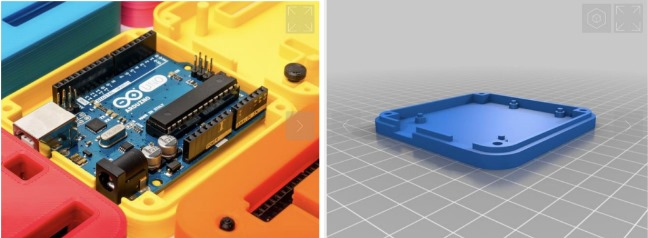
\includegraphics[width=1\linewidth]{P3/img/image1.jpg}
    \caption{Referensi Desain Enclosure}
    \label{fig:Referensi Desain Enclosure}
\end{figure}

\begin{figure}[H]
    \centering
    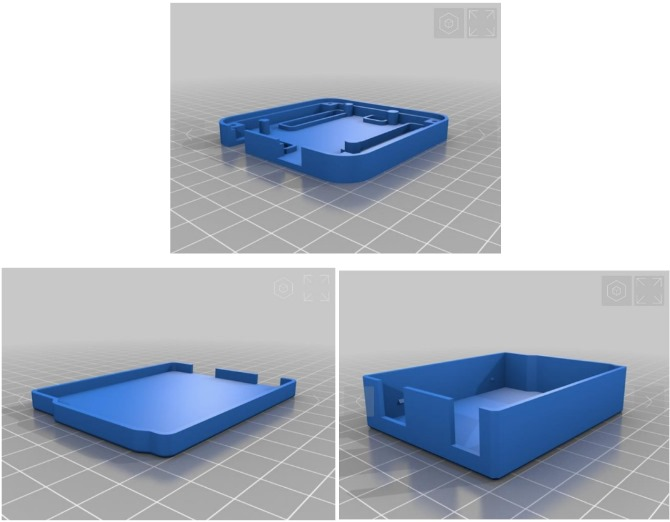
\includegraphics[width=1\linewidth]{P3/img/image2.jpg}
    \caption{Komponen Enclosure}
    \label{fig:Komponen Enclosure}
\end{figure}

Kesalahan yang seringkali dijumpai pada proses desain 3D yaitu alur kerja yang terlalu repetitive ataupun
bertele-tele, karena sebenarnya fitur software banyak yang kurang di-explore sehingga saat
menggunakan software, fitur yang digunakan kurang membantu pengerjaan desain atau bahkan
memperlamanya. Untuk itu hendaknya mencari referensi, dokumentasi, ataupun inspirasi yang terdapat
di sekitar seperti lego, laptop, ataupun projektil lain yang dapat ditiru, amati, dan modifikasi desainnya.

\section{Tugas Pendahuluan}
\begin{enumerate}
    \item Buat satu desain kubus pada fusion 360 seperti pada gambar dibawah ini
        \begin{figure}[H]
            \centering
            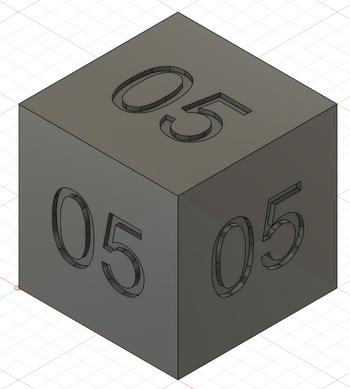
\includegraphics[width=0.25\linewidth]{P3/img/soal1.png}
            \caption{Tugas Pendahuluan}
            \label{fig:Tugas Pendahuluan}
        \end{figure}
    \item Install Ultimaker CURA
\end{enumerate}

\section{Alat dan Komponen}
\subsection{Alat}
\begin{enumerate}
    \item Laptop yang telah terinstall Autodesk Fusion 360
    \item Laptop yang telah terinstall Ultimaker CURA untuk print 3d
    \item Mouse
\end{enumerate}

\section{Eksperimen 1: Membuat Enclosure PCB}
Buatlah enclosure dari PCB yang disediakan. Enclosure harus terbagi setidaknya menjadi dua bagian yaitu
\textbf{“Bawah”} sebagai tumpuan PCB dan \textbf{“Atas”} sebagai penutup enclosure. Enclosure juga harus memiliki
lubang power untuk tempat memberi tegangan PCB.
\begin{enumerate}
    \item Sebelum mendesain, upload lah file model 3D dengan type file .stp yang sudah disediakan. Untuk
    mengupload model klik \textbf{“Upload”} di panel sebelah kiri.
        \begin{figure}[H]
            \centering
            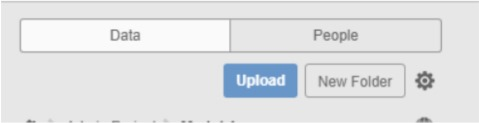
\includegraphics[width=0.5\linewidth]{P3/img/image3.jpg}
            \caption{Upload}
            \label{fig:Upload}
        \end{figure}

    \item Untuk memulai mendesain Enclosure klik pada \textbf{“file”} dan klik pada \textbf{“New Design”} atau juga saat
    membuka fusion otomatis new design akan terbuka sendirinya. Setelah new design terbuka klik
    save (ctrl + s) dan beri nama terserah.
        \begin{figure}[H]
            \centering
            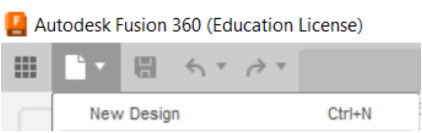
\includegraphics[width=0.5\linewidth]{P3/img/image4.jpg}
            \caption{New Design}
            \label{fig:New Design}
        \end{figure}

    \item Langkah selanjutnya adalah memasukan model PCB 3D yang sudah diupload sebelumnya. Untuk
    memasukan model PCB klik kanan pada model tersebut lalu klik \textbf{“Insert into current Design”}.
        \begin{figure}[H]
            \centering
            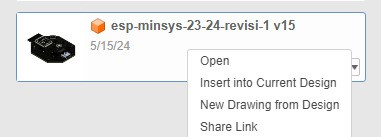
\includegraphics[width=0.5\linewidth]{P3/img/Insert to Current Design 2.jpg}
            \caption{Insert Into Curret Design}
            \label{fig:Insert Into Curret Design}
        \end{figure}

        \begin{figure}[H]
            \centering
            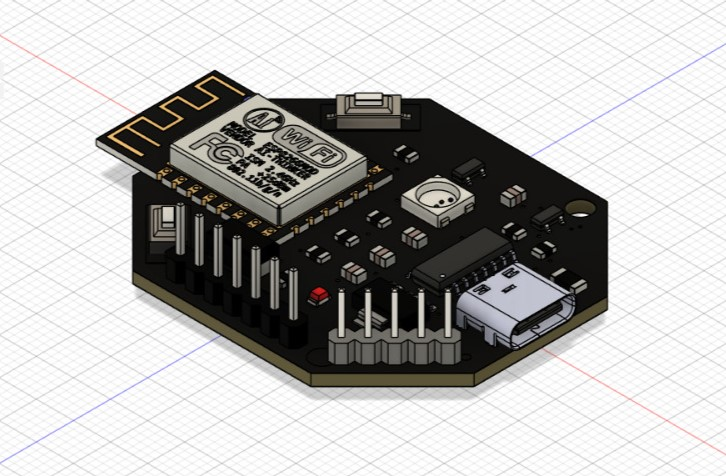
\includegraphics[width=0.5\linewidth]{P3/img/Insert PCB.jpg}
            \caption{Sudah di Insert}
            \label{fig:Sudah di Insert}
        \end{figure}

    \item Saat membuat enclosure terdapat beberapa tools yang tersedia. Berikut beberapa tools yang
    akan sering digunakan dalam pembuatan enclosure:
        \begin{figure}[H]
            \centering
            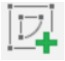
\includegraphics[width=0.1\linewidth]{P3/img/image6.jpg}
            \caption{Sketch}
            \label{fig:Sketch}
        \end{figure}
        
        \textbf{Sketch}: menggambar sketsa 2D dari bentuk yang akan dibuat. Sketsa ini dapat digunakan
        bersama Extrude untuk membuat nya menjadi body 3D.
            
        \begin{figure}[H]
            \centering
            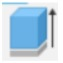
\includegraphics[width=0.1\linewidth]{P3/img/image7.jpg}
            \caption{Extrude}
            \label{fig:Extrude}
        \end{figure}

        \textbf{Extrude}: Mengatur ukuran dari body. Bisa digunakan untuk memperpanjang atau
        memperpendek suatu sisi dari body.
        \begin{figure}[H]
            \centering
            
\includegraphics[width=0.1\linewidth]{P3/img/image8.jpg}
            \caption{Combine}
            \label{fig:Combine}
        \end{figure}
    
        \textbf{Combine}: Menggabungkan dua atau lebih body menjadi satu.
            
        \begin{figure}[H]
            \centering
            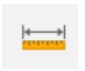
\includegraphics[width=0.1\linewidth]{P3/img/image9.jpg}
            \caption{Measure}
            \label{fig:Measure}
        \end{figure}
        \textbf{Measure}: Mengukur body Model 3D
            
        \begin{figure}[H]
                \centering
                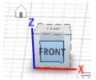
\includegraphics[width=0.1\linewidth]{P3/img/image10.jpg}
                \caption{Camera}
                \label{fig:Camera}
            \end{figure}
        \textbf{Camera}: Menggerakan Camera (Dapat juga menggunakan shift+ klik scroll mouse + gerak
        mouse).

    \item PBC yang dimasukan digunakan sebagai referensi ukuran enclosure yang akan dibuat. Gunakan
    Tools \textbf{“Measure”} untuk mengukur dimensi dari PCB.
    \item Setelah didapat ukuran PCB Gunakan Tools \textbf{“Sketch”} untuk membuat sketsa 2D yang nanti nya
    akan digunakan Tools \textbf{“Extrude”} untuk mengubahnya menjadi body 3D.
    \item Body-body yang terpisah dapat digabungkan menjadi satu menggunakan Tools \textbf{“Combine”}.
    \item Untuk menvigasi dalam ruang 3D dapat digunakan \textbf{“Camera”} untuk melihat dan mebangung
    dari segala sisi/sumbu.
    \item Buatlah setidak nya dua bagian \textbf{“Bawah”} sebagai tumpuan PCB dan \textbf{“Atas”} sebagai penutup
    enclosure.
    \item Buatlah sekreatif mungkin.
\end{enumerate}

\begin{figure}[H]
    \centering
    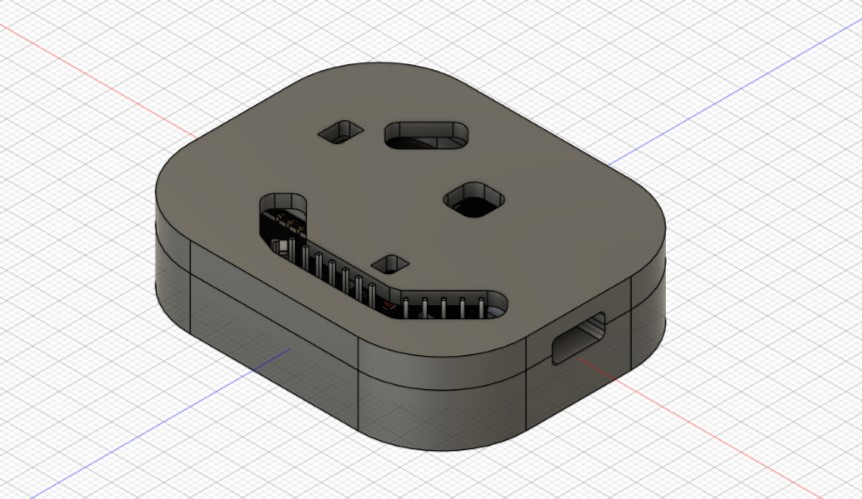
\includegraphics[width=0.5\linewidth]{P3/img/Enclosure Close 2.jpg}
    \caption{Enclosure close}
    \label{fig:Enclosure close}
\end{figure}

\begin{figure}[H]
    \centering
    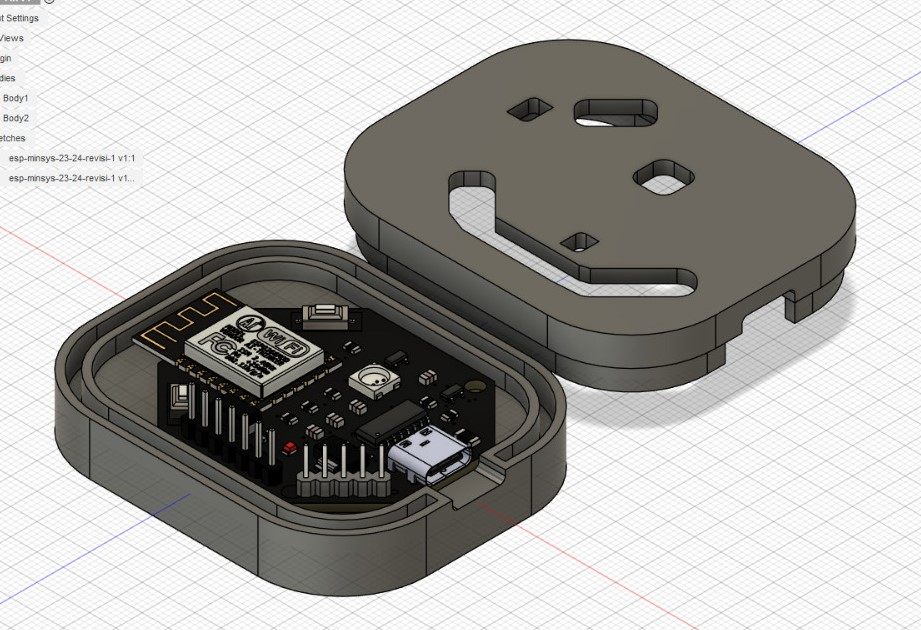
\includegraphics[width=0.5\linewidth]{P3/img/Enclosure Open 2.jpg}
    \caption{Enclosure open}
    \label{fig:Enclosure open}
\end{figure}
\section{Eksperimen 2: Mencetak Enclosure PCB}
Setelah Enclosure PCB telah dibuat, saatnya mencetaknya menggunakan Ulitmaker CURA. 
\begin{enumerate}
    \item Sebelum mencetaknya, eksport enclosure secara terpisah bagian
     \textbf{“Bawah”} dan \textbf{“Atas”} dengan format file .STL.
     \begin{figure}[H]
        \centering
        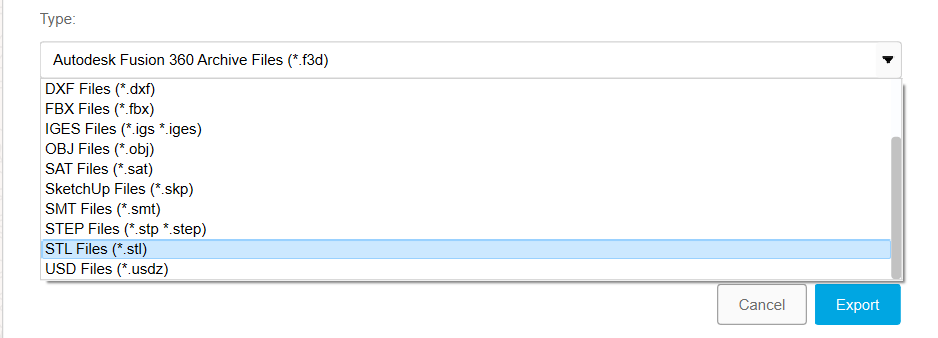
\includegraphics[width=0.5\linewidth]{P3/img/Eksport.png}
        \caption{Eksport}
        \label{fig:Eksport}
    \end{figure}
    \item Setelah mengeksportnya, buka ultimaker cura dan klik \textbf{“File”} kemudian 
    \textbf{“Open file”} dan pilih kedua file yang tadi sudah di eksport, 
    lalu posisikan agar tidak tergabung satu sama lain.
     \begin{figure}[H]
        \centering
        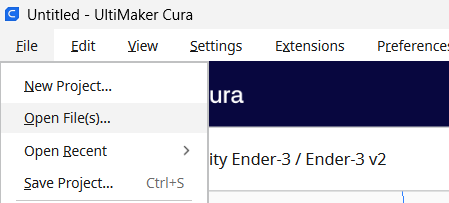
\includegraphics[width=0.5\linewidth]{P3/img/Open File.png}
        \caption{Open File}
        \label{fig:Open File}
    \end{figure}
    \item Untuk yang bagian \textbf{“Atas”}, rotasikan 180 derajat agar bisa dicetak dengan support yang minim.
    \begin{figure}[H]
       \centering
       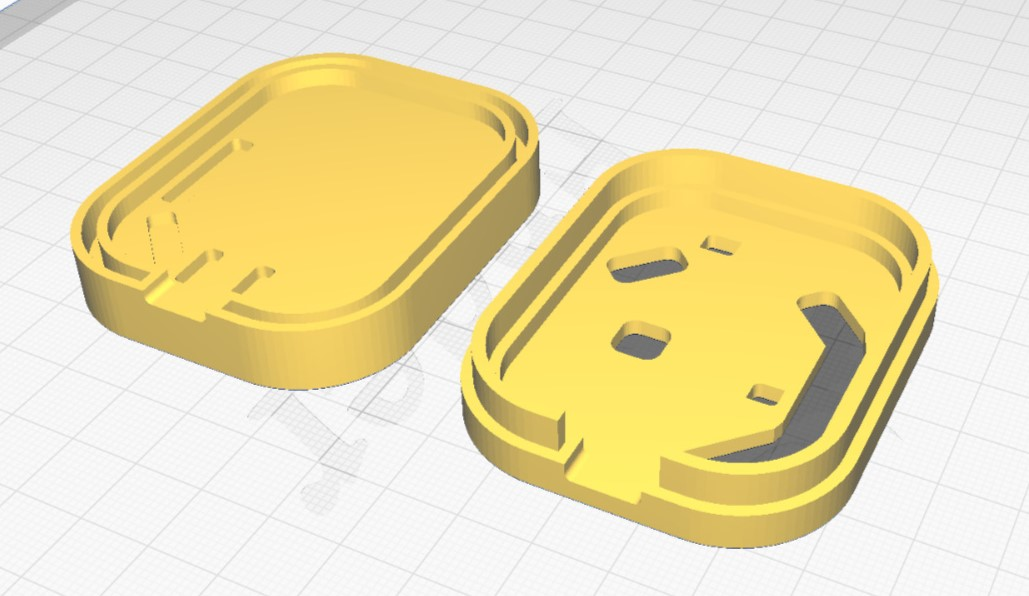
\includegraphics[width=0.5\linewidth]{P3/img/Enclosure 3D 2.jpg}
       \caption{Enclosure bagian 'Atas' Sudah dibalik}
       \label{fig:Enclosure}
   \end{figure}
    \item Saatnya melakukan konfigurasi sebelum enclosure dicetak, tekan bagian standart quality pada bagian kanan atas 
    lalu settingan yang kita ubah hanya bagian walls, infill, material, cooling, support,dan build plate adhesion.
    \begin{figure}[H]
        \centering
        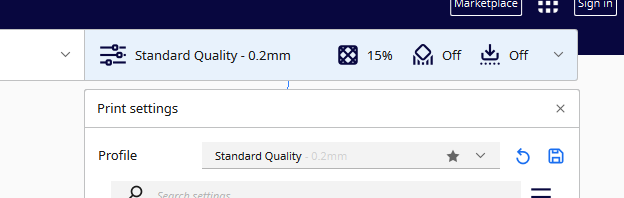
\includegraphics[width=0.5\linewidth]{P3/img/settings.png}
        \caption{Print settings}
        \label{fig:Settings}
    \end{figure}
    \item Pada bagian walls, digunakan untuk mengatur ketebalan dindingnya dan berapa banyak lapisan,
    bagian yang diubah adalah "Wall Thickness" menjadi 0.8mm dan "Wall Line Count" menjadi 2 sesuai gambar dibawah. 
    \begin{figure}[H]
        \centering
        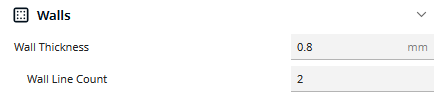
\includegraphics[width=0.5\linewidth]{P3/img/Setting walls.png}
        \caption{Setting Walls}
        \label{fig:Settings walls}
    \end{figure}

    \item Pada bagian infill, digunakan untuk mengatur kerapatan dinidng dalamnya dan juga bentuknya bagaimana,
    yang diubah adalah "Infill Density" menjadi 20\% dan "Infill Pattern" menggunakan Lines sesuai gambar dibawah.
    \begin{figure}[H]
        \centering
        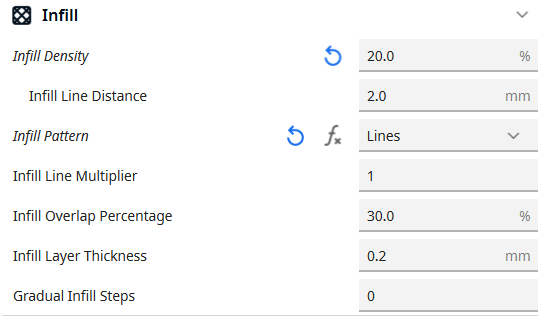
\includegraphics[width=0.5\linewidth]{P3/img/Settings infill 2.png}
        \caption{Setting Infill}
        \label{fig:Settings Infill}
    \end{figure}
    \item Pada bagian material, digunakan untuk mengubah suhu untuk memanaskan filamennya dan juga suhu pada platenya,
    yang diubah adalah "Printing Temperature" menjadi 205\degree C dan "Build Plate Temperature" menjadi 60\degree C sesuai gambar dibawah.
    \begin{figure}[H]
        \centering
        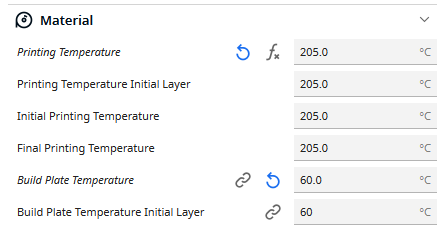
\includegraphics[width=0.5\linewidth]{P3/img/Settings material.png}
        \caption{Settings Material}
        \label{fig:Settings Material}
    \end{figure}
    \item Pada bagian cooling, digunakan untuk mengatur seberapa cepat kecepatan kipasnya,
    yang diubah adalah "Fan Speed" menjadi 100\% sesuai gambar dibawah.
    \begin{figure}[H]
        \centering
        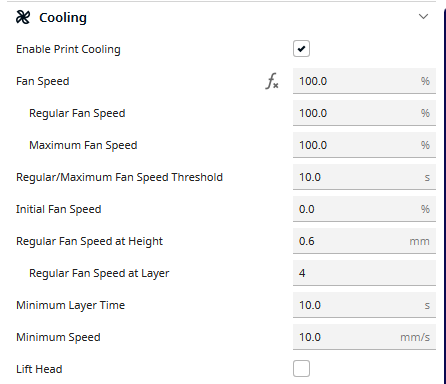
\includegraphics[width=0.5\linewidth]{P3/img/Settings cooling.png}
        \caption{Settings cooling}
        \label{fig:Settings Cooling}
    \end{figure}
    \item Pada bagian build plate adhesion, digunakan sebagai batasan area 3D printnya
    yang diubah adalah "Build Plate Adhesion Type" menggunakan Brim dan "Brim Line Count" menjadi 20 sesuai gambar dibawah.
    \begin{figure}[H]
        \centering
        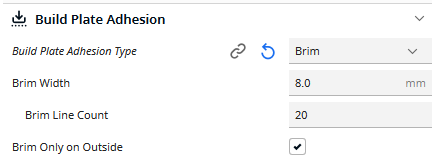
\includegraphics[width=0.7\linewidth]{P3/img/Settings Build.png}
        \caption{Settings Build Plate Adhesion}
        \label{fig:Settings Build Plate Adhesion}
    \end{figure}
    \item Setelah melakukan settingan untuk 3D printing, tekan \textbf{"Slice"} lalu \textbf{"Preview"} untuk melihat lapisan lapisan pada 3D model dan
    bagaimana 3D printer melakukan printing.
    \begin{figure}[H]
        \centering
        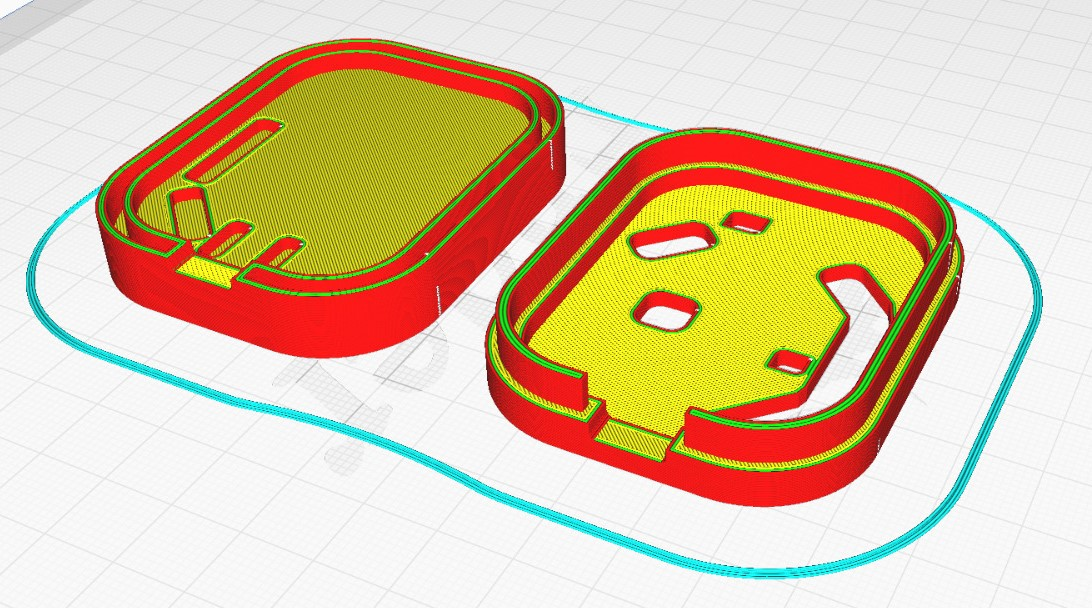
\includegraphics[width=0.6\linewidth]{P3/img/Hasil slice 2.jpg}
        \caption{Hasil Slice}
        \label{fig:Hasil Slice}
    \end{figure}
    \item Jika sudah selesai semua, simpan hasil kalian dengan tekan \textbf{"Save to Disk"}, simpan dengan nama file \textbf{"Kelompok xx"} menggunakan tipe file .gcode.
    \begin{figure}[H]
        \centering
        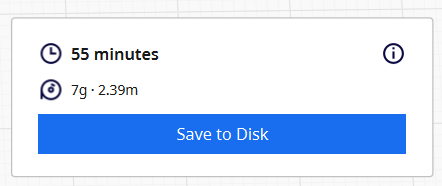
\includegraphics[width=0.5\linewidth]{P3/img/Save file.png}
        \caption{Save file}
        \label{fig:Save file}
    \end{figure}
\end{enumerate}